\documentclass[conference]{IEEEtran}
\usepackage[utf8]{inputenc}
\usepackage[T1]{fontenc}
\usepackage[spanish,es-tabla,es-nodecimaldot,es-noshorthands]{babel}
\usepackage{amsmath,amssymb}
\usepackage{graphicx}
\usepackage{cite}
\usepackage{url}
\usepackage{listings}
\usepackage{xcolor}
\usepackage{placeins}
\usepackage{tikz}
\usetikzlibrary{shapes.geometric,arrows.meta,positioning}

\lstset{
  language=Matlab,
  basicstyle=\ttfamily\scriptsize,
  keywordstyle=\color{blue!70!black}\bfseries,
  commentstyle=\color{green!45!black},
  stringstyle=\color{violet},
  numbers=left, numberstyle=\tiny\color{gray},
  breaklines=true, frame=single, columns=fullflexible,
  showstringspaces=false, tabsize=4,
  literate={á}{{\'a}}1 {é}{{\'e}}1 {í}{{\'i}}1 {ó}{{\'o}}1 {ú}{{\'u}}1 {ñ}{{\~n}}1
}

\begin{document}

\title{Influencia de los operadores y par\'ametros de un algoritmo gen\'etico en la soluci\'on de tres problemas de optimizaci\'on}

\author{\IEEEauthorblockN{Fernando Andr\'es Zuluaga Botero}
\IEEEauthorblockA{Bioingenier\'ia, Unidad 3 -- Optimizaci\'on metaheur\'istica\\
Universidad Cat\'olica de Oriente, Rionegro, Colombia\\
fernando.zuluaga3427@uco.net.co}}

\maketitle

\begin{abstract}
Se implement\'o en MATLAB un algoritmo gen\'etico (AG) gen\'erico y se aplic\'o a tres problemas de minimizaci\'on: el problema del viajero entre 13 ubicaciones del oriente antioque\~no, la funci\'on Ackley modificada y un problema de pol\'itica de inventarios con restricci\'on de igualdad. Para cada problema se programaron la funci\'on objetivo, la generaci\'on de la poblaci\'on inicial, un operador de cruce apropiado a su representaci\'on (cruce por orden, BLX-$\alpha$ y cruce aritm\'etico) y un operador de mutaci\'on; adem\'as, se implementaron tres m\'etodos de selecci\'on comunes (elitismo, torneo y ruleta). Se realizaron cuatro estudios encadenados, con 10 ejecuciones por escenario: m\'etodo de selecci\'on, n\'umero de iteraciones, estrategia de mutaci\'on y n\'umero de dimensiones de la funci\'on Ackley. La selecci\'on por elitismo obtuvo los mejores resultados en los tres casos; la ruleta, en cambio, present\'o una presi\'on selectiva insuficiente. El AG encontr\'o el recorrido \'optimo del viajero (509 min, verificado con programaci\'on din\'amica) en 4 de 10 ejecuciones y alcanz\'o el m\'inimo de Ackley ($3-e$) con errores del orden de $10^{-9}$ en 3 dimensiones, pero su exactitud se degrad\'o r\'apidamente al aumentar las dimensiones. En el problema de inventarios, la mutaci\'on result\'o decisiva: el valor esperado de pedidos no atendidos pas\'o de $886.8$ sin mutaci\'on a $337.8$ con $P_m=1$ y una magnitud del 20\,\% del rango.
\end{abstract}

\begin{IEEEkeywords}
Algoritmo gen\'etico, optimizaci\'on metaheur\'istica, problema del viajero, funci\'on Ackley, control de inventarios, selecci\'on, cruce, mutaci\'on.
\end{IEEEkeywords}

% =====================================================================
\section{Introducci\'on}
La naturaleza ha inspirado a disciplinas muy distintas: los mec\'anicos han observado aves y mam\'iferos para dise\~nar veh\'iculos m\'as aerodin\'amicos, y los ingenieros han visto en los enjambres de abejas o en las colonias de hormigas modelos de organizaci\'on capaces de resolver problemas complejos sin un control central. Detr\'as de estas adaptaciones hay millones de a\~nos de evoluci\'on, que favorece a los individuos mejor adaptados a su entorno. Este proceso inspir\'o a John H. Holland, cuyo trabajo culmin\'o en 1975 con una de las obras fundacionales de los algoritmos gen\'eticos \cite{holland}: un m\'etodo que imita algunos mecanismos de la evoluci\'on para optimizar ya no organismos, sino modelos matem\'aticos y f\'isicos.

Los algoritmos de optimizaci\'on metaheur\'istica se han aplicado al dise\~no de ejes de transmisi\'on \cite{ejes}, turbinas hidr\'aulicas \cite{turbina1,turbina2}, microrredes \cite{montoya,grisales} y redes de sensores \cite{sensores}, entre otros problemas en los que el espacio de b\'usqueda es grande, hay m\'ultiples variables y restricciones, o la relaci\'on entre las variables y el desempe\~no es compleja. Su eficacia se debe a estrategias que exploran el espacio de soluciones sin recorrerlo exhaustivamente \cite{boussaid}.

Un algoritmo gen\'etico, sin embargo, no es un procedimiento \'unico: su comportamiento depende de la representaci\'on de los individuos, de los operadores de selecci\'on, cruce y mutaci\'on, y de par\'ametros como el tama\~no de la poblaci\'on o el n\'umero de generaciones. Adem\'as, por su naturaleza estoc\'astica, una sola ejecuci\'on no basta para caracterizar una configuraci\'on; es necesario repetir los experimentos y analizar la calidad, la variabilidad y el costo computacional de los resultados \cite{latorre}.

En este trabajo se construy\'o un AG gen\'erico en MATLAB y se estudi\'o experimentalmente la influencia de sus operadores y par\'ametros en tres problemas: el problema del viajero (combinatorio), la funci\'on Ackley (continua, con muchos m\'inimos locales y dimensi\'on variable) y un problema real de pol\'itica de inventarios (continuo y con restricciones).

% =====================================================================
\section{Marco te\'orico}
\subsection{Problemas de optimizaci\'on}
Optimizar consiste en hallar el vector $\vec{X}^*$ que minimiza (o maximiza) una funci\'on $F$ dentro de su dominio v\'alido $\Omega$:
\begin{equation}
F(\vec{X}^*) = \min_{\vec{X}\in\Omega} F(\vec{X}),
\end{equation}
\begin{equation}
\Omega = \left\{\vec{X}\in \mathrm{dom}(f) \mid g_i(\vec{X})\le 0,\; h_j(\vec{X})=0 \;\; \forall i,j \right\},
\end{equation}
donde $f$ es la funci\'on objetivo o de aptitud (\emph{fitness}), $g_i$ son las restricciones de desigualdad y $h_j$ las de igualdad. En los tres problemas estudiados se busca un m\'inimo.

\subsection{Algoritmo gen\'etico}
El AG trabaja con una poblaci\'on de soluciones candidatas (individuos). Cada individuo tiene un genotipo (su codificaci\'on: una permutaci\'on o un vector real) y un fenotipo (la soluci\'on que representa), cuya calidad se mide con la funci\'on de aptitud. En cada generaci\'on se \emph{seleccionan} los individuos que se reproducen, se \emph{cruzan} para crear descendientes que combinan la informaci\'on de sus padres y se \emph{mutan} algunos de ellos para introducir variaciones aleatorias que mantengan la diversidad \cite{holland,goldberg}. El proceso se repite durante un n\'umero determinado de generaciones.

\subsection{M\'etodos de selecci\'on}
\begin{itemize}
\item \textbf{Elitismo:} se ordenan los individuos por aptitud y se conserva la mejor mitad.
\item \textbf{Torneo:} se forman grupos aleatorios de 4 individuos (sin repetir individuos entre grupos) y de cada grupo pasan los 2 mejores.
\item \textbf{Ruleta:} cada individuo se escoge con una probabilidad proporcional a su aptitud. En minimizaci\'on, esta probabilidad es inversamente proporcional al valor de la funci\'on objetivo:
\begin{equation}
P(\vec{X}_i) = \frac{1/f(\vec{X}_i)}{\sum_{j=1}^{n} 1/f(\vec{X}_j)}.
\label{eq:ruleta}
\end{equation}
\end{itemize}
Estos m\'etodos difieren en su \emph{presi\'on selectiva}, es decir, en qu\'e tanto favorecen a los mejores individuos \cite{goldbergdeb}. Una presi\'on alta acelera la convergencia pero puede reducir la diversidad; una presi\'on baja mantiene la diversidad pero hace m\'as lenta la b\'usqueda.

\subsection{M\'etricas de desempe\~no}
La exactitud se mide con la ra\'iz del error cuadr\'atico medio respecto al \'optimo conocido,
\begin{equation}
\mathrm{RMSE}=\sqrt{\frac{1}{n_{p}}\sum_{i=1}^{n_{p}}\left(Y_i-f(\vec{X}^*)\right)^2},
\end{equation}
donde $Y_i$ es el mejor valor de la $i$-\'esima ejecuci\'on y $n_p$ el n\'umero de ejecuciones. La precisi\'on se mide con la desviaci\'on est\'andar de los $Y_i$, y el costo computacional con el tiempo de ejecuci\'on.

% =====================================================================
\section{Metodolog\'ia}
Todo el c\'odigo se implement\'o en MATLAB R2026a (ver Anexo). Cada operador es una funci\'on independiente y un \'unico programa, \texttt{algoritmo\_genetico.m}, recibe los operadores de cada problema como \emph{function handles}.

\subsection{Funciones objetivo}
\subsubsection{Problema del viajero}
Cada ubicaci\'on se identifica con un n\'umero del 1 al 13, en el orden de la Tabla~I de la gu\'ia (UCO $=1$, Rionegro $=2$, \dots, Guatap\'e $=13$), y un recorrido es una lista con esos n\'umeros. La funci\'on \texttt{f\_viajero} suma los tiempos $T_{ij}$ entre ubicaciones consecutivas \emph{incluyendo el regreso al punto de partida}, de modo que el recorrido es un ciclo cerrado. As\'i, la lista $[1,2,\dots,13]$ da $641+89=730$~min. La matriz de tiempos no es sim\'etrica ($T_{ij}\neq T_{ji}$), por lo que el sentido del recorrido s\'i importa. Si la lista no es una permutaci\'on de $1,\dots,13$, se suma una penalizaci\'on de 10\,000~min, mayor que la suma de todos los tiempos de la tabla (9\,534~min).

Aunque $13!\approx6.2\times10^{9}$ recorridos hacen inviable la fuerza bruta, el \'optimo exacto s\'i puede obtenerse con el algoritmo de programaci\'on din\'amica de Held y Karp \cite{heldkarp}, de complejidad $O(n^2 2^n)$. Se implement\'o \'unicamente como referencia para medir la exactitud del AG: el recorrido \'optimo tarda \textbf{509~min} (UCO $\to$ Rionegro $\to$ El Retiro $\to$ La Ceja $\to$ La Uni\'on $\to$ El Carmen $\to$ Santuario $\to$ Cocorn\'a $\to$ Guatap\'e $\to$ El Pe\~nol $\to$ Marinilla $\to$ San Vicente $\to$ Guarne $\to$ UCO).

\subsubsection{Funci\'on Ackley}
Se implement\'o la versi\'on modificada de la gu\'ia \cite{ackley}:
\begin{equation}
f(\vec{X}) = -a\,e^{-b\sqrt{\frac{1}{d}\sum_{i=1}^{d}x_i^2}} - e^{\frac{1}{d}\sum_{i=1}^{d}\cos(c\,x_i)} + a + 3,
\end{equation}
con $a=20$, $b=0.2$, $c=2\pi$ y $x_i\in[-10,10]$. Su m\'inimo global est\'a en $\vec{X}=\vec{0}$ y vale $3-e\approx0.281718$, lo que se verific\'o num\'ericamente para $d=1,2,3,10$ y 100.

\subsubsection{Pol\'itica de inventarios}
El individuo es $\vec{X}=[Q_1..Q_5,\,S_1..S_5,\,K_1..K_5]$ y la funci\'on objetivo es el n\'umero esperado de pedidos no atendidos por a\~no \cite{gardner,chen}:
\begin{equation}
Z=\sum_{i=1}^{5}\frac{D_i}{Q_i}\int_{S_i+K_i}^{\infty}\frac{x_i-S_i-K_i}{m_i\sqrt{2\pi}\sigma_i}e^{-\frac12\left(\frac{x_i-\mu_i}{\sigma_i}\right)^2}dx_i ,
\end{equation}
con los par\'ametros de la Tabla~II de la gu\'ia. La integral se calcul\'o con el comando \texttt{integral} de MATLAB tras el cambio de variable $x_i=R_i+t$, con $R_i=S_i+K_i$ y $t\in[0,\infty)$. Esto permite integrar los cinco \'items en una sola llamada (opci\'on \texttt{ArrayValued}), con un costo de 0.73~ms por evaluaci\'on. Como verificaci\'on, se compar\'o con la funci\'on de p\'erdida de la distribuci\'on normal, $\sigma_i[\phi(z)-z(1-\Phi(z))]$ con $z=(R_i-\mu_i)/\sigma_i$: la diferencia m\'axima en 200 individuos fue de $1.3\times10^{-7}$.

Las restricciones son $0\le S_i\le c_{1,i}$, $0\le K_i\le c_{2,i}$ y la igualdad
\begin{equation}
\sum_{i=1}^{5}\left(\frac{Q_i}{2}+S_i\right)=I=8000.
\label{eq:igualdad}
\end{equation}
Para $Q_i$, cuyo l\'imite superior en la gu\'ia es $\infty$, se asumi\'o $Q_i\in[1,\;2I]=[1,\;16\,000]$. El l\'imite inferior evita la divisi\'on por cero y el superior corresponde al caso extremo en que todo el presupuesto de inventario se asigna a un solo art\'iculo sin stock de seguridad: por (\ref{eq:igualdad}), $Q_i/2$ nunca puede superar $I$.

\subsection{Poblaciones iniciales}
\begin{itemize}
\item \textbf{Viajero} (\texttt{pob\_viajero}): $n$ permutaciones aleatorias de $1,\dots,13$ generadas con \texttt{randperm}, por lo que no hay elementos repetidos.
\item \textbf{Ackley} (\texttt{pob\_ackley}): matriz $n\times d$ de valores uniformes en el intervalo $[-10,10]$.
\item \textbf{Inventarios} (\texttt{pob\_inventario}): se generan 14 variables. $S_i$ y $K_i$ son uniformes en sus l\'imites. $Q_1,\dots,Q_4$ se toman como fracciones aleatorias (distribuci\'on de Dirichlet) del presupuesto que queda libre, $I-\sum S_i$. Finalmente, $Q_5$ se despeja de (\ref{eq:igualdad}). Este procedimiento garantiza $Q_5>0$ sin necesidad de descartar individuos, y se verific\'o que todos los individuos cumplen (\ref{eq:igualdad}) exactamente y respetan los l\'imites.
\end{itemize}

\subsection{Operadores de cruce}
Se escogi\'o un cruce adecuado a la representaci\'on de cada problema. En todos los casos, cada pareja de padres genera dos hijos.
\begin{itemize}
\item \textbf{Viajero, cruce por orden (OX)} \cite{larranaga}: se eligen dos puntos de corte; el hijo copia el segmento central de un padre y completa las dem\'as posiciones con las ciudades del otro padre en el orden en que aparecen, sin repetir. Los hijos siempre son permutaciones v\'alidas y conservan el orden relativo de las ciudades, que es lo que determina el tiempo del recorrido.
\item \textbf{Ackley, BLX-$\alpha$} \cite{herrera}: para cada gen, con $C_{\min}=\min(p_1,p_2)$, $C_{\max}=\max(p_1,p_2)$ e $I=C_{\max}-C_{\min}$, el hijo toma un valor uniforme en $[C_{\min}-\alpha I,\;C_{\max}+\alpha I]$, con $\alpha=0.5$, y luego se recorta al dominio. Al permitir valores fuera del intervalo entre los padres, el operador tambi\'en explora.
\item \textbf{Inventarios, cruce aritm\'etico} \cite{herrera}: con $\lambda\sim U(0,1)$, los hijos son $h_1=\lambda p_1+(1-\lambda)p_2$ y $h_2=(1-\lambda)p_1+\lambda p_2$. Como son combinaciones convexas de padres factibles, los hijos cumplen autom\'aticamente la igualdad lineal (\ref{eq:igualdad}) y los l\'imites de caja. Por eso este cruce es especialmente apropiado para este problema.
\end{itemize}

\subsection{Operadores de mutaci\'on}
Cada hijo muta con probabilidad $P_m$ (por individuo), que es un par\'ametro modificable.
\begin{itemize}
\item \textbf{Viajero:} se intercambian dos posiciones escogidas al azar (\emph{swap}), por lo que el hijo sigue siendo una permutaci\'on.
\item \textbf{Ackley:} a un gen escogido al azar se le suma $r\sim\mathcal{N}(0,\sigma_m^2)$ y el resultado se recorta a $[-10,10]$.
\item \textbf{Inventarios:} se escoge una de las 14 variables independientes y se le suma $r\sim\mathcal{N}(0,(\sigma_r\cdot\text{rango})^2)$, donde el rango es el ancho del intervalo permitido para esa variable. As\'i se tienen en cuenta las distintas escalas de las variables. Luego se recalcula $Q_5$ con (\ref{eq:igualdad}); si queda fuera de sus l\'imites, se descarta la mutaci\'on y se intenta de nuevo, hasta un m\'aximo de 10 intentos.
\end{itemize}

\subsection{Esquema generacional}
En cada generaci\'on (Fig.~\ref{fig:flujo}) se selecciona la mitad de la poblaci\'on, se forman parejas al azar, cada pareja produce dos hijos y los hijos se mutan. La nueva poblaci\'on est\'a formada por los padres seleccionados y sus hijos, de modo que su tama\~no no cambia. El algoritmo guarda el mejor individuo encontrado hasta el momento, porque con la ruleta el mejor individuo puede no ser seleccionado.

\begin{figure}[!t]
\centering
\begin{tikzpicture}[node distance=4.5mm, every node/.style={font=\scriptsize},
  caja/.style={draw, rounded corners, fill=blue!6, minimum width=36mm, minimum height=5.5mm, align=center},
  dec/.style={draw, diamond, aspect=2.4, fill=orange!10, inner sep=1pt, align=center},
  flecha/.style={-{Stealth[length=2mm]}}]
\node[caja] (ini) {Poblaci\'on inicial ($n$ individuos)};
\node[caja, below=of ini] (eva) {Evaluaci\'on de la aptitud $f(\vec{X})$};
\node[caja, below=of eva] (sel) {Selecci\'on de $n/2$ padres};
\node[caja, below=of sel] (cru) {Cruce: $n/2$ hijos};
\node[caja, below=of cru] (mut) {Mutaci\'on de los hijos ($P_m$)};
\node[caja, below=of mut] (nue) {Nueva poblaci\'on = padres + hijos};
\node[dec, below=of nue] (fin) {¿Iteraciones\\completas?};
\node[caja, below=of fin, fill=green!8] (res) {Mejor individuo $\hat{X}$};
\draw[flecha] (ini) -- (eva); \draw[flecha] (eva) -- (sel);
\draw[flecha] (sel) -- (cru); \draw[flecha] (cru) -- (mut);
\draw[flecha] (mut) -- (nue); \draw[flecha] (nue) -- (fin);
\draw[flecha] (fin) -- node[right]{S\'i} (res);
\draw[flecha] (fin.east) -- ++(9mm,0) |- node[pos=0.25,right]{No} (eva.east);
\end{tikzpicture}
\caption{Diagrama de flujo del algoritmo gen\'etico implementado.}
\label{fig:flujo}
\end{figure}

\subsection{Dise\~no experimental}
Se us\'o una poblaci\'on de $n=60$ individuos (m\'ultiplo de 4, como exige el torneo) y 10 ejecuciones por escenario, con semillas $1,\dots,10$ (\texttt{rng(k)}) para que los resultados sean reproducibles. Los estudios 1 a 3 se hicieron con Ackley en $d=3$. La configuraci\'on base fue de 100 iteraciones y $P_m=0.2$, con $\sigma_m=0.5$ en Ackley y $\sigma_r=0.05$ en inventarios. Los estudios se encadenaron de la siguiente forma:
\begin{enumerate}
\item \textbf{Selecci\'on:} se comparan los tres m\'etodos con 100 iteraciones y se escoge el de menor promedio (si hay empate, el de menor desviaci\'on).
\item \textbf{Iteraciones:} se prueban 10, 20, 30, 50, 100, 150 y 200 iteraciones con el m\'etodo ganador. Se escoge el menor n\'umero de iteraciones cuyo promedio est\'e a menos del 1\,\% del mejor promedio.
\item \textbf{Mutaci\'on:} se var\'ia $P_m\in\{0,\,0.05,\,0.1,\,0.2,\,0.4,\,0.7,\,1\}$; luego, con el mejor $P_m>0$, se var\'ia la magnitud de la mutaci\'on ($\sigma_m\in\{0.1,0.5,1,2\}$ en Ackley y $\sigma_r\in\{0.01,0.05,0.1,0.2\}$ en inventarios). $P_m=0$ se usa como escenario de control y no se considera en la elecci\'on.
\item \textbf{Dimensiones:} se optimiza Ackley con $d=2,3,10,20,50$ y 100, usando la configuraci\'on elegida en los estudios anteriores.
\end{enumerate}
En las tablas, $t$ es el tiempo promedio por ejecuci\'on, $f(\hat{X})$ el mejor valor de las 10 ejecuciones, $\hat{X}$ el individuo que lo obtuvo, y ``Prom.'' y ``Desv.'' el promedio y la desviaci\'on est\'andar de los mejores valores de cada ejecuci\'on. En el viajero se reporta adem\'as el RMSE respecto al \'optimo exacto.

% =====================================================================
\section{Resultados y an\'alisis}

\subsection{Estudio 1: m\'etodo de selecci\'on}
% Generado automaticamente por generar_salidas.m
\begin{table}[!t]
\centering
\scriptsize
\setlength{\tabcolsep}{2.5pt}
\caption{Estudio 1 -- problema del viajero: m\'etodo de selecci\'on (100 iteraciones).}
\label{tab:t1v}
\begin{tabular}{lrrrrrl}
\hline
M\'etodo & $t$ (ms) & $f(\hat{X})$ & Prom. & Desv. & RMSE$^*$ & $\hat{X}$ (ruta) \\
\hline
Elitismo & 36.4 & 509 & 514.1 & 6.19 & 7.78 & 13-12-5-10-6-1-2-7-3-9-4-8-11 \\
Torneo & 31.2 & 509 & 518.2 & 7.89 & 11.86 & 2-7-3-9-4-8-11-13-12-5-10-6-1 \\
Ruleta & 29.5 & 554 & 578.4 & 12.49 & 70.40 & 5-3-9-7-1-2-10-6-4-8-11-13-12 \\
\hline
\multicolumn{7}{l}{$^*$RMSE respecto al \'optimo exacto (509 min, Held-Karp).}
\end{tabular}
\end{table}

% Generado automaticamente por generar_salidas.m
\begin{table*}[!t]
\centering
\scriptsize
\setlength{\tabcolsep}{2.5pt}
\caption{Estudio 1 -- funci\'on Ackley ($d=3$): m\'etodo de selecci\'on (100 iteraciones).}
\label{tab:t1a}
\begin{tabular}{lrrrrrl}
\hline
M\'etodo & $t$ (ms) & $f(\hat{X})$ & Prom. & Desv. & RMSE & $\hat{X}$ \\
\hline
Elitismo & 9.65 & 0.281718 & 0.281718 & $1.34{\times}10^{-9}$ & $1.77{\times}10^{-9}$ & ($-2.90{\times}10^{-11}$, $1.22{\times}10^{-11}$, $9.30{\times}10^{-12}$) \\
Torneo & 10.06 & 0.281718 & 0.281718 & $6.57{\times}10^{-9}$ & $9.41{\times}10^{-9}$ & ($-9.23{\times}10^{-11}$, $2.78{\times}10^{-10}$, $-9.28{\times}10^{-11}$) \\
Ruleta & 5.73 & 0.285186 & 0.290279 & $6.48{\times}10^{-3}$ & 0.011 & ($1.15{\times}10^{-4}$, $-5.60{\times}10^{-4}$, $-1.37{\times}10^{-3}$) \\
\hline
\end{tabular}
\end{table*}

% Generado automaticamente por generar_salidas.m
\begin{table*}[!t]
\centering
\scriptsize
\setlength{\tabcolsep}{3pt}
\caption{Estudio 1 -- inventarios: m\'etodo de selecci\'on (100 iteraciones). Valores monetarios en miles de COP.}
\label{tab:t1i}
\begin{tabular}{lrrrrlll}
\hline
M\'etodo & $t$ (s) & $f(\hat{X})$ & Prom. & Desv. & $\hat{Q}$ & $\hat{S}$ & $\hat{K}$ \\
\hline
Elitismo & 1.63 & 502.30 & 558.72 & 32.69 & (437, 3547, 2703, 2778, 1784) & (65, 501, 510, 202, 1097) & (353, 1685, 4607, 1170, 2993) \\
Torneo & 1.62 & 484.16 & 564.06 & 45.88 & (414, 4221, 2432, 1567, 1952) & (40, 744, 649, 431, 845) & (413, 1177, 4985, 1483, 2946) \\
Ruleta & 1.64 & 829.66 & 913.74 & 59.86 & (896, 2297, 2831, 2230, 2953) & (51, 503, 473, 518, 851) & (287, 1138, 4301, 620, 2258) \\
\hline
\end{tabular}
\end{table*}


Las Tablas~\ref{tab:t1v}, \ref{tab:t1a} y \ref{tab:t1i} y la Fig.~\ref{fig:conv} muestran que el \textbf{elitismo} obtuvo el menor promedio en los tres problemas, seguido de cerca por el torneo. En el viajero, el elitismo encontr\'o el \'optimo exacto de 509~min en 4 de 10 ejecuciones y el torneo en 3; el promedio del elitismo (514.1~min) est\'a apenas un 1\,\% por encima del \'optimo. En Ackley ambos alcanzaron $3-e$ con errores de $10^{-9}$. En inventarios la diferencia entre ambos fue peque\~na frente a la dispersi\'on: el torneo encontr\'o el mejor valor individual (484.2) y el elitismo tuvo el mejor promedio (558.7) y la menor desviaci\'on.

La \textbf{ruleta} fue claramente la peor en los tres casos. Seg\'un (\ref{eq:ruleta}), la probabilidad de selecci\'on depende de $1/f$, y cuando los valores de $f$ de la poblaci\'on son parecidos (por ejemplo, recorridos de 520 y 560~min) sus probabilidades casi no se diferencian. La presi\'on selectiva resulta entonces casi nula y la b\'usqueda se comporta de forma cercana a un muestreo aleatorio \cite{goldbergdeb}. Adem\'as, al ser con reemplazo, la ruleta puede dejar por fuera al mejor individuo, cosa que no ocurre con el elitismo ni con el torneo de 4 (el mejor siempre queda entre los 2 primeros de su grupo). En inventarios esto es evidente: con ruleta, $Z$ se estanca cerca de 910 desde las primeras generaciones (Fig.~\ref{fig:conv}). La ruleta s\'olo fue m\'as r\'apida porque ordena menos, pero la diferencia de tiempo es despreciable. Se eligi\'o el elitismo para los estudios siguientes en los tres problemas.

\begin{figure}[!t]
\centering
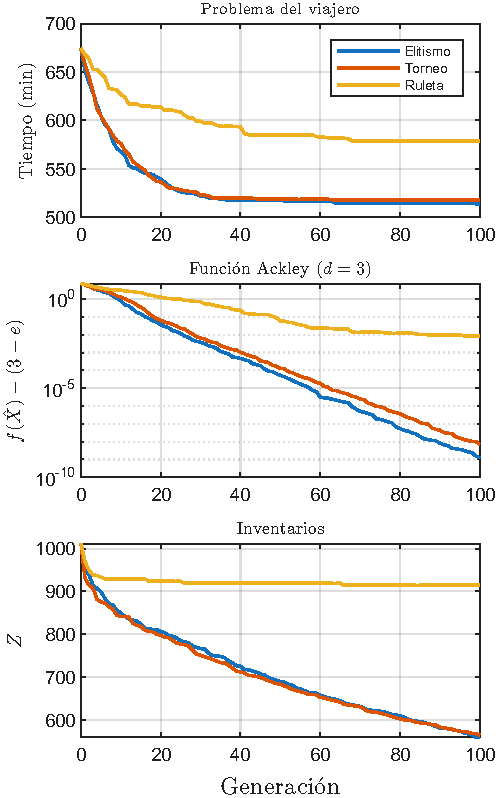
\includegraphics[width=\columnwidth]{figuras/convergencia_seleccion.pdf}
\caption{Convergencia promedio (10 ejecuciones) del mejor valor encontrado para cada m\'etodo de selecci\'on, con 100 iteraciones. En Ackley se grafica el error respecto al \'optimo en escala logar\'itmica.}
\label{fig:conv}
\end{figure}

\subsection{Estudio 2: n\'umero de iteraciones}
% Generado automaticamente por generar_salidas.m
\begin{table}[!t]
\centering
\scriptsize
\setlength{\tabcolsep}{2.5pt}
\caption{Estudio 2 -- problema del viajero: n\'umero de iteraciones (selecci\'on por elitismo).}
\label{tab:t2v}
\begin{tabular}{lrrrrrl}
\hline
Iter. & $t$ (ms) & $f(\hat{X})$ & Prom. & Desv. & RMSE$^*$ & $\hat{X}$ (ruta) \\
\hline
10 & 8.5 & 551 & 567.9 & 13.69 & 60.32 & 9-3-7-2-1-8-11-5-12-13-6-10-4 \\
20 & 7.5 & 510 & 539.8 & 19.33 & 35.85 & 8-11-13-12-5-2-1-10-6-7-3-9-4 \\
30 & 10.2 & 509 & 521.5 & 13.69 & 18.02 & 12-5-10-6-1-2-7-3-9-4-8-11-13 \\
50 & 13.9 & 509 & 517.5 & 8.37 & 11.63 & 13-12-5-10-6-1-2-7-3-9-4-8-11 \\
100 & 26.4 & 509 & 514.1 & 6.19 & 7.78 & 13-12-5-10-6-1-2-7-3-9-4-8-11 \\
150 & 38.2 & 509 & 514.1 & 6.19 & 7.78 & 13-12-5-10-6-1-2-7-3-9-4-8-11 \\
200 & 56.1 & 509 & 514.1 & 6.19 & 7.78 & 13-12-5-10-6-1-2-7-3-9-4-8-11 \\
\hline
\multicolumn{7}{l}{$^*$RMSE respecto al \'optimo exacto (509 min, Held-Karp).}
\end{tabular}
\end{table}

% Generado automaticamente por generar_salidas.m
\begin{table*}[!t]
\centering
\scriptsize
\setlength{\tabcolsep}{2.5pt}
\caption{Estudio 2 -- funci\'on Ackley ($d=3$): n\'umero de iteraciones (selecci\'on por elitismo).}
\label{tab:t2a}
\begin{tabular}{lrrrrrl}
\hline
Iter. & $t$ (ms) & $f(\hat{X})$ & Prom. & Desv. & RMSE & $\hat{X}$ \\
\hline
10 & 2.66 & 0.449046 & 1.055537 & 0.456 & 0.886 & (-0.013, -0.032, 0.039) \\
20 & 0.89 & 0.288317 & 0.317418 & 0.016 & 0.039 & ($-1.75{\times}10^{-3}$, $-1.64{\times}10^{-3}$, $-1.45{\times}10^{-3}$) \\
30 & 1.31 & 0.282235 & 0.285437 & $2.64{\times}10^{-3}$ & $4.48{\times}10^{-3}$ & ($4.64{\times}10^{-5}$, $1.56{\times}10^{-4}$, $-1.53{\times}10^{-4}$) \\
50 & 2.57 & 0.281729 & 0.281770 & $6.87{\times}10^{-5}$ & $8.32{\times}10^{-5}$ & ($1.25{\times}10^{-6}$, $3.45{\times}10^{-6}$, $2.83{\times}10^{-6}$) \\
100 & 4.06 & 0.281718 & 0.281718 & $1.34{\times}10^{-9}$ & $1.77{\times}10^{-9}$ & ($-2.90{\times}10^{-11}$, $1.22{\times}10^{-11}$, $9.30{\times}10^{-12}$) \\
150 & 7.59 & 0.281718 & 0.281718 & $4.74{\times}10^{-11}$ & $4.74{\times}10^{-11}$ & ($-1.15{\times}10^{-16}$, $-1.91{\times}10^{-16}$, $2.19{\times}10^{-16}$) \\
200 & 8.78 & 0.281718 & 0.281718 & $4.72{\times}10^{-11}$ & $4.72{\times}10^{-11}$ & ($-4.57{\times}10^{-18}$, $-3.51{\times}10^{-18}$, $-1.46{\times}10^{-16}$) \\
\hline
\end{tabular}
\end{table*}

% Generado automaticamente por generar_salidas.m
\begin{table*}[!t]
\centering
\scriptsize
\setlength{\tabcolsep}{3pt}
\caption{Estudio 2 -- inventarios: n\'umero de iteraciones (selecci\'on por elitismo). Valores monetarios en miles de COP.}
\label{tab:t2i}
\begin{tabular}{lrrrrlll}
\hline
Iter. & $t$ (s) & $f(\hat{X})$ & Prom. & Desv. & $\hat{Q}$ & $\hat{S}$ & $\hat{K}$ \\
\hline
10 & 0.22 & 750.40 & 848.82 & 49.11 & (1100, 3202, 2390, 2519, 2169) & (59, 488, 524, 195, 1044) & (352, 1031, 3726, 851, 2574) \\
20 & 0.34 & 718.04 & 805.99 & 39.59 & (1039, 3208, 2701, 2501, 1928) & (60, 491, 524, 200, 1036) & (349, 1334, 3719, 854, 2490) \\
30 & 0.53 & 677.32 & 765.84 & 37.76 & (1037, 3216, 2679, 2501, 1940) & (60, 491, 524, 200, 1039) & (351, 1303, 3934, 921, 2660) \\
50 & 0.82 & 599.32 & 689.34 & 41.61 & (440, 3369, 2699, 2775, 2060) & (66, 498, 523, 202, 1039) & (350, 1510, 3782, 925, 3000) \\
100 & 1.66 & 502.30 & 558.72 & 32.69 & (437, 3547, 2703, 2778, 1784) & (65, 501, 510, 202, 1097) & (353, 1685, 4607, 1170, 2993) \\
150 & 4.71 & 431.75 & 470.45 & 23.70 & (437, 3595, 2721, 2778, 1663) & (72, 501, 450, 207, 1172) & (406, 1898, 4974, 1388, 2983) \\
200 & 4.59 & 399.16 & 418.74 & 12.14 & (328, 3576, 2721, 2772, 1573) & (74, 569, 297, 233, 1342) & (416, 1993, 4976, 1494, 2991) \\
\hline
\end{tabular}
\end{table*}


Como era de esperarse, el promedio y la desviaci\'on disminuyen al aumentar las iteraciones, mientras que el tiempo crece de forma aproximadamente lineal (Tablas~\ref{tab:t2v}--\ref{tab:t2i}). El comportamiento, sin embargo, fue diferente en cada problema:
\begin{itemize}
\item \textbf{Viajero:} con 30 iteraciones ya se encontr\'o el \'optimo en una ejecuci\'on. A partir de 100 iteraciones los resultados son id\'enticos (514.1~min en promedio), porque la poblaci\'on converge a un solo recorrido y la \'unica fuente de variaci\'on que queda es la mutaci\'on. En las 6 ejecuciones que no llegaron al \'optimo, el algoritmo qued\'o atrapado en un \'optimo local. Seg\'un el criterio definido se escogieron \textbf{50 iteraciones} (517.5~min, a menos del 1\,\% del mejor promedio).
\item \textbf{Ackley ($d=3$):} con 10 iteraciones el error promedio es de 0.77. Con 50 iteraciones cae a $10^{-4}$ y con 100 a $10^{-9}$. Se escogieron \textbf{50 iteraciones}.
\item \textbf{Inventarios:} $Z$ sigue disminuyendo hasta 200 iteraciones (de 848.8 con 10 a 418.7 con 200), lo que indica que el algoritmo no ha convergido. Es el problema m\'as dif\'icil: tiene 14 variables continuas con escalas muy distintas y cada evaluaci\'on requiere integrar. Se escogieron \textbf{200 iteraciones}, el m\'aximo del estudio. Las diferencias de tiempo que no son proporcionales a las iteraciones (por ejemplo, 150 frente a 200) se deben a la variabilidad de la carga del computador.
\end{itemize}

\subsection{Estudio 3: estrategia de mutaci\'on}
% Generado automaticamente por generar_salidas.m
\begin{table}[!t]
\centering
\scriptsize
\setlength{\tabcolsep}{2.5pt}
\caption{Estudio 3 -- problema del viajero: probabilidad de mutaci\'on $P_m$ (elitismo, 50 iteraciones).}
\label{tab:t3v}
\begin{tabular}{lrrrrl}
\hline
$P_m$ & $f(\hat{X})$ & Prom. & Desv. & RMSE$^*$ & $\hat{X}$ (ruta) \\
\hline
0.00 & 509 & 525.9 & 12.64 & 20.72 & 12-5-10-6-1-2-7-3-9-4-8-11-13 \\
0.05 & 509 & 522.3 & 9.49 & 16.06 & 13-12-5-10-6-1-2-7-3-9-4-8-11 \\
0.10 & 510 & 522.3 & 9.19 & 15.90 & 5-2-1-10-6-7-3-9-4-8-11-13-12 \\
0.20 & 509 & 517.5 & 8.37 & 11.63 & 13-12-5-10-6-1-2-7-3-9-4-8-11 \\
0.40 & 509 & 516.0 & 6.91 & 9.59 & 4-8-11-13-12-5-10-6-1-2-7-3-9 \\
0.70 & 509 & 519.4 & 8.60 & 13.22 & 9-4-8-11-13-12-5-10-6-1-2-7-3 \\
1.00 & 512 & 524.9 & 10.97 & 19.00 & 5-10-6-1-2-7-9-3-4-8-11-13-12 \\
\hline
\multicolumn{6}{l}{$^*$RMSE respecto al \'optimo exacto (509 min, Held-Karp).}
\end{tabular}
\end{table}

% Generado automaticamente por generar_salidas.m
\begin{table*}[!t]
\centering
\scriptsize
\setlength{\tabcolsep}{2.5pt}
\caption{Estudio 3 -- funci\'on Ackley ($d=3$): probabilidad $P_m$ y magnitud $\sigma_m$ de la mutaci\'on (elitismo, 50 iteraciones).}
\label{tab:t3a}
\begin{tabular}{lrrrrl}
\hline
$P_m$ / $\sigma_m$ & $f(\hat{X})$ & Prom. & Desv. & RMSE & $\hat{X}$ \\
\hline
0.00 / 0.5 & 0.281722 & 0.281729 & $6.94{\times}10^{-6}$ & $1.29{\times}10^{-5}$ & ($1.07{\times}10^{-6}$, $1.02{\times}10^{-6}$, $-2.51{\times}10^{-7}$) \\
0.05 / 0.5 & 0.281722 & 0.281735 & $2.06{\times}10^{-5}$ & $2.57{\times}10^{-5}$ & ($-5.36{\times}10^{-7}$, $6.64{\times}10^{-7}$, $-1.28{\times}10^{-6}$) \\
0.10 / 0.5 & 0.281723 & 0.281996 & $7.65{\times}10^{-4}$ & $7.77{\times}10^{-4}$ & ($1.79{\times}10^{-7}$, $-1.02{\times}10^{-6}$, $-2.03{\times}10^{-6}$) \\
0.20 / 0.5 & 0.281729 & 0.281770 & $6.87{\times}10^{-5}$ & $8.32{\times}10^{-5}$ & ($1.25{\times}10^{-6}$, $3.45{\times}10^{-6}$, $2.83{\times}10^{-6}$) \\
0.40 / 0.5 & 0.281776 & 0.282203 & $5.57{\times}10^{-4}$ & $7.17{\times}10^{-4}$ & ($-9.59{\times}10^{-6}$, $7.00{\times}10^{-6}$, $2.22{\times}10^{-5}$) \\
0.70 / 0.5 & 0.282477 & 0.284995 & $3.32{\times}10^{-3}$ & $4.54{\times}10^{-3}$ & ($-7.32{\times}10^{-5}$, $3.09{\times}10^{-4}$, $8.07{\times}10^{-5}$) \\
1.00 / 0.5 & 0.294778 & 0.322898 & 0.018 & 0.045 & ($-4.97{\times}10^{-7}$, $1.66{\times}10^{-3}$, $-5.17{\times}10^{-3}$) \\
0.05 / 0.1 & 0.281721 & 0.281741 & $2.16{\times}10^{-5}$ & $3.06{\times}10^{-5}$ & ($-9.64{\times}10^{-7}$, $-4.06{\times}10^{-7}$, $9.68{\times}10^{-7}$) \\
0.05 / 1.0 & 0.281721 & 0.281733 & $1.02{\times}10^{-5}$ & $1.77{\times}10^{-5}$ & ($1.14{\times}10^{-6}$, $-1.70{\times}10^{-7}$, $5.35{\times}10^{-7}$) \\
0.05 / 2.0 & 0.281721 & 0.281791 & $1.37{\times}10^{-4}$ & $1.49{\times}10^{-4}$ & ($8.02{\times}10^{-7}$, $-2.03{\times}10^{-7}$, $-7.28{\times}10^{-7}$) \\
\hline
\end{tabular}
\end{table*}

% Generado automaticamente por generar_salidas.m
\begin{table*}[!t]
\centering
\scriptsize
\setlength{\tabcolsep}{3pt}
\caption{Estudio 3 -- inventarios: probabilidad $P_m$ y magnitud relativa $\sigma_r$ de la mutaci\'on (elitismo, 200 iteraciones). Valores monetarios en miles de COP.}
\label{tab:t3i}
\begin{tabular}{lrrrlll}
\hline
$P_m$ / $\sigma_r$ & $f(\hat{X})$ & Prom. & Desv. & $\hat{Q}$ & $\hat{S}$ & $\hat{K}$ \\
\hline
0.00 / 0.05 & 767.58 & 886.83 & 54.72 & (1160, 3256, 2406, 2550, 2087) & (58, 481, 499, 181, 1051) & (360, 1037, 3768, 860, 2396) \\
0.05 / 0.05 & 498.47 & 557.72 & 44.42 & (979, 3199, 2658, 1795, 2327) & (45, 674, 460, 492, 850) & (365, 1279, 4959, 1492, 3000) \\
0.10 / 0.05 & 452.59 & 487.21 & 23.92 & (400, 3732, 2700, 1499, 2099) & (55, 675, 603, 503, 949) & (362, 1585, 4781, 1495, 2975) \\
0.20 / 0.05 & 399.16 & 418.74 & 12.14 & (328, 3576, 2721, 2772, 1573) & (74, 569, 297, 233, 1342) & (416, 1993, 4976, 1494, 2991) \\
0.40 / 0.05 & 369.83 & 384.15 & 12.38 & (282, 3711, 3265, 1993, 1835) & (59, 567, 18, 615, 1196) & (410, 1993, 4995, 1492, 2997) \\
0.70 / 0.05 & 349.83 & 364.28 & 8.80 & (173, 3780, 2984, 1642, 1323) & (32, 772, 64, 737, 1445) & (490, 1999, 4999, 1500, 2998) \\
1.00 / 0.05 & 348.51 & 355.61 & 6.47 & (203, 4143, 3056, 1451, 1403) & (22, 610, 16, 800, 1425) & (489, 1999, 5000, 1499, 2999) \\
1.00 / 0.01 & 500.89 & 580.91 & 46.21 & (344, 4179, 2549, 1799, 2025) & (31, 688, 513, 415, 905) & (395, 847, 4987, 1498, 2968) \\
1.00 / 0.10 & 337.21 & 340.10 & 2.09 & (94, 3089, 2955, 1504, 1325) & (26, 1195, 2, 798, 1495) & (500, 2000, 5000, 1500, 3000) \\
1.00 / 0.20 & 336.16 & 337.83 & 1.92 & (118, 2936, 3219, 1423, 1262) & (21, 1200, 0, 800, 1500) & (500, 2000, 5000, 1500, 3000) \\
\hline
\end{tabular}
\end{table*}


El efecto de $P_m$ (Fig.~\ref{fig:pm}) depende del problema:
\begin{itemize}
\item \textbf{Viajero:} la curva tiene forma de ``U''. Sin mutaci\'on el promedio es de 525.9~min: el cruce OX solo recombina lo que ya existe en la poblaci\'on, y el elitismo pierde diversidad r\'apidamente. Con $P_m=0.4$ se obtuvo el mejor promedio (516.0~min), la menor desviaci\'on (6.9) y 4 de 10 ejecuciones en el \'optimo. Con $P_m=1$ el resultado empeora (524.9~min), porque se perturban casi todos los hijos y se destruyen buenas subrutas.
\item \textbf{Ackley ($d=3$):} con $P_m\le0.2$ todos los resultados son pr\'acticamente iguales (errores promedio entre $10^{-5}$ y $10^{-4}$), pues el BLX-$\alpha$ ya explora lo suficiente en 3 dimensiones. Con $P_m\ge0.7$ la mutaci\'on aleja a los individuos del \'optimo cuando la poblaci\'on ya est\'a cerca de \'el, y con $P_m=1$ el RMSE sube a 0.045. La magnitud $\sigma_m$ tuvo poco efecto; se eligi\'o $P_m=0.05$ y $\sigma_m=1$.
\item \textbf{Inventarios:} la mutaci\'on es decisiva. Sin ella, $Z=886.8$; con $P_m=1$ y $\sigma_r=0.05$, $Z=355.6$; y al aumentar la magnitud a $\sigma_r=0.2$, $Z=337.8$ con una desviaci\'on de solo 1.9. La raz\'on es estructural: el cruce aritm\'etico produce combinaciones convexas de los padres, as\'i que la poblaci\'on nunca puede salir del ``envolvente'' de la poblaci\'on inicial, que adem\'as se contrae en cada generaci\'on. La mutaci\'on es el \'unico operador que puede llevar las variables a los l\'imites. Se eligi\'o $P_m=1$ y $\sigma_r=0.2$, los valores extremos de la malla, por lo que conviene explorar valores mayores en trabajos futuros.
\end{itemize}

La mejor pol\'itica de inventario encontrada ($Z=336.2$) tiene una interpretaci\'on clara. Todos los $K_i$ quedaron en su l\'imite superior: $K_i$ no aparece en la restricci\'on (\ref{eq:igualdad}) y aumentarlo siempre reduce $Z$, as\'i que el algoritmo lo lleva al m\'aximo, como era de esperarse. El stock de seguridad se concentr\'o en los \'items 2, 4 y 5 (en su l\'imite), mientras que $S_3\approx0$ y $S_1\approx21$. El \'item 3 tiene el mayor valor por pedido ($m_3=900$) y el \'item 1 las menores ventas ($D_1=12\,000$), de modo que invertir en su stock de seguridad reduce poco el n\'umero de pedidos no atendidos. En cambio, $Q_3$ es alto: para el \'item de mayores ventas conviene hacer pedidos grandes y pocas veces.

\begin{figure}[!t]
\centering
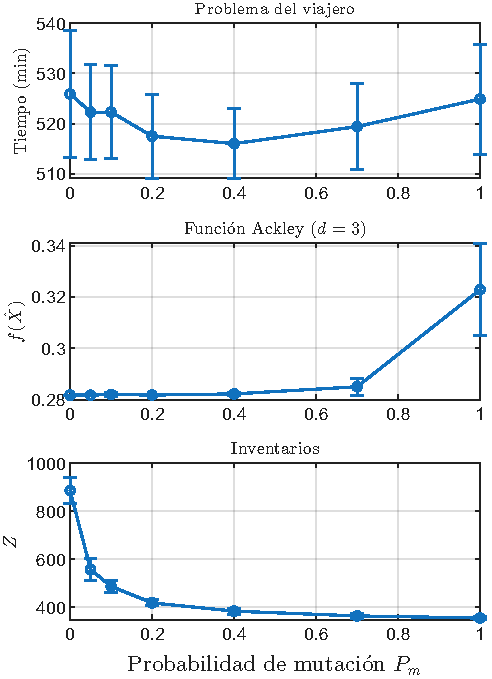
\includegraphics[width=\columnwidth]{figuras/efecto_pm.pdf}
\caption{Promedio y desviaci\'on est\'andar (barras) del mejor valor en funci\'on de la probabilidad de mutaci\'on $P_m$.}
\label{fig:pm}
\end{figure}

\subsection{Estudio 4: n\'umero de dimensiones de Ackley}
% Generado automaticamente por generar_salidas.m
\begin{table}[!t]
\centering
\scriptsize
\setlength{\tabcolsep}{3pt}
\caption{Estudio 4 -- funci\'on Ackley: n\'umero de dimensiones (elitismo, 50 iteraciones, $P_m=0.05$, $\sigma_m=1.0$).}
\label{tab:t4a}
\begin{tabular}{rrrrrrr}
\hline
$d$ & $t$ (ms) & $f(\hat{X})$ & Prom. & Desv. & RMSE & $\|\hat{X}\|_\infty$ \\
\hline
2 & 2.15 & 0.2817 & 0.2817 & $3.11{\times}10^{-7}$ & $3.51{\times}10^{-7}$ & $3.38{\times}10^{-10}$ \\
3 & 2.01 & 0.2817 & 0.2817 & $1.02{\times}10^{-5}$ & $1.77{\times}10^{-5}$ & $1.14{\times}10^{-6}$ \\
10 & 2.34 & 0.3323 & 0.4823 & 0.339 & 0.379 & 0.020 \\
20 & 2.97 & 1.6879 & 2.0827 & 0.342 & 1.830 & 0.320 \\
50 & 4.15 & 4.6696 & 5.4080 & 0.498 & 5.148 & 1.665 \\
100 & 6.87 & 7.5101 & 8.0978 & 0.343 & 7.823 & 5.557 \\
\hline
\end{tabular}
\end{table}


Con la configuraci\'on elegida (elitismo, 50 iteraciones, $P_m=0.05$, $\sigma_m=1$), el AG encontr\'o el m\'inimo global en $d=2$ y $d=3$ (RMSE de $10^{-7}$ y $10^{-5}$). A partir de $d=10$ la exactitud se degrada r\'apidamente (Tabla~\ref{tab:t4a} y Fig.~\ref{fig:dim}): el RMSE pasa de 0.38 en $d=10$ a 7.82 en $d=100$, y la mayor coordenada del mejor individuo pasa de 0.02 a 5.6, es decir, el algoritmo termina lejos del origen y atrapado en m\'inimos locales. Hay tres causas principales:
\begin{enumerate}
\item El espacio de b\'usqueda crece exponencialmente con $d$, pero la poblaci\'on (60) y las iteraciones (50) se mantuvieron fijas.
\item La mutaci\'on modifica solo un gen por individuo, lo que en 100 dimensiones es una perturbaci\'on m\'inima.
\item La configuraci\'on se ajust\'o en $d=3$, donde el problema es f\'acil.
\end{enumerate}
El tiempo creci\'o poco (de 2 a 7~ms) porque la evaluaci\'on de Ackley est\'a vectorizada. Por lo tanto, tendr\'ia sentido aumentar el tama\~no de la poblaci\'on y el n\'umero de iteraciones para problemas de alta dimensi\'on. Los individuos completos de este estudio est\'an en el archivo \texttt{estudio4\_mejores\_individuos.csv} del repositorio.

\begin{figure}[!t]
\centering
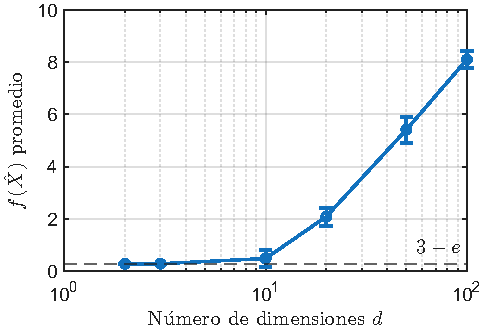
\includegraphics[width=\columnwidth]{figuras/dimensiones.pdf}
\caption{Promedio y desviaci\'on est\'andar del mejor valor de Ackley en funci\'on del n\'umero de dimensiones. La l\'inea discontinua es el \'optimo $3-e$.}
\label{fig:dim}
\end{figure}

% =====================================================================
\FloatBarrier
\section{Conclusiones}
\begin{itemize}
\item La selecci\'on por elitismo obtuvo los mejores promedios en los tres problemas, con el torneo muy cerca. La selecci\'on por ruleta con probabilidad inversa al fitness tuvo una presi\'on selectiva insuficiente, porque las aptitudes de la poblaci\'on son muy parecidas, y fue la peor en todos los casos.
\item El n\'umero adecuado de iteraciones depende del problema: 50 fueron suficientes para el viajero y para Ackley en 3 dimensiones, mientras que en inventarios el algoritmo segu\'ia mejorando con 200. Al no conocerse el \'optimo, la estabilizaci\'on de la curva de convergencia y la reducci\'on de la desviaci\'on son los criterios pr\'acticos para decidir.
\item La importancia de la mutaci\'on depende del operador de cruce. En el viajero conviene un valor intermedio ($P_m=0.4$); en Ackley ($d=3$) casi no tiene efecto, porque BLX-$\alpha$ ya explora; y en inventarios es indispensable, porque el cruce aritm\'etico no puede salir de la envolvente convexa de la poblaci\'on.
\item El cruce aritm\'etico permiti\'o manejar la restricci\'on de igualdad del problema de inventarios sin penalizaciones, ya que conserva la factibilidad por construcci\'on.
\item El AG encontr\'o el recorrido \'optimo del viajero (509~min, verificado con Held-Karp) en el 40\,\% de las ejecuciones, pero su exactitud en Ackley cae con la dimensi\'on si no se escalan la poblaci\'on, las iteraciones y la mutaci\'on. Esto confirma que la configuraci\'on de un AG debe ajustarse a cada problema y que su evaluaci\'on exige m\'ultiples ejecuciones y an\'alisis estad\'istico.
\end{itemize}

% =====================================================================
\section*{Anexo: c\'odigos}
Los c\'odigos en MATLAB, los resultados de los cuatro estudios y los archivos fuente de este informe est\'an disponibles en el repositorio \url{https://github.com/upfernan/algoritmo-genetico}. Para reproducir los resultados se ejecutan, en este orden, \texttt{pruebas}, \texttt{experimentos(1)} a \texttt{experimentos(4)} y \texttt{generar\_salidas} desde la carpeta \texttt{codigo}.

% =====================================================================
\begin{thebibliography}{99}
\bibitem{holland} J. H. Holland, \emph{Adaptation in Natural and Artificial Systems: An Introductory Analysis with Applications to Biology, Control, and Artificial Intelligence}. Ann Arbor, MI: University of Michigan Press, 1975.
\bibitem{ejes} M. A. Rodriguez-Cabal, J. D. Betancur-G\'omez, L. F. Grisales-Nore\~na, O. D. Montoya, and D. Hincapie, ``Optimal design of transmission shafts using a Vortex Search Algorithm,'' \emph{Arabian Journal for Science and Engineering}, vol. 46, no. 4, pp. 3293--3300, 2021.
\bibitem{turbina1} A. J. P\'erez Rodr\'iguez, J. A. Sierra Del R\'io, and D. A. Hincapi\'e-Zuluaga, ``Optimizaci\'on del rendimiento de una turbina Michell Banki utilizando algoritmos PSO y BHO,'' in \emph{Congreso Internacional de Ingenier\'ia con Impacto Social}, Medell\'in, Colombia, 2019, pp. 30--34.
\bibitem{turbina2} A. J. Perez-Rodriguez, J. Sierra-Del Rio, L. F. Grisales-Nore\~na, and S. Galvis, ``Optimization of the efficiency of a Michell-Banki turbine through the variation of its geometrical parameters using a PSO algorithm,'' \emph{WSEAS Transactions on Heat and Mass Transfer}, vol. 17, pp. 45--53, 2022.
\bibitem{montoya} O. D. Montoya, W. Gil-Gonz\'alez, and L. F. Grisales-Nore\~na, ``Vortex search algorithm for optimal power flow analysis in DC resistive networks with CPLs,'' \emph{IEEE Transactions on Circuits and Systems II: Express Briefs}, vol. 67, no. 8, pp. 1439--1443, 2020.
\bibitem{grisales} L. F. Grisales-Nore\~na, D. G. Montoya, and C. A. Ramos-Paja, ``Optimal sizing and location of distributed generators based on PBIL and PSO techniques,'' \emph{Energies}, vol. 11, no. 4, pp. 1--27, 2018.
\bibitem{sensores} E. H. Houssein, M. R. Saad, Y. Djenouri, G. Hu, A. A. Ali, and H. Shaban, ``Metaheuristic algorithms and their applications in wireless sensor networks: Review, open issues, and challenges,'' \emph{Cluster Computing}, vol. 27, no. 10, pp. 13643--13673, 2024.
\bibitem{boussaid} I. Boussa\"id, J. Lepagnot, and P. Siarry, ``A survey on optimization metaheuristics,'' \emph{Information Sciences}, vol. 237, pp. 82--117, 2013.
\bibitem{latorre} A. LaTorre, D. Molina, E. Osaba, J. Poyatos, J. Del Ser, and F. Herrera, ``A prescription of methodological guidelines for comparing bio-inspired optimization algorithms,'' \emph{Swarm and Evolutionary Computation}, vol. 67, p. 100973, 2021.
\bibitem{goldberg} D. E. Goldberg, \emph{Genetic Algorithms in Search, Optimization, and Machine Learning}. Reading, MA: Addison-Wesley, 1989.
\bibitem{goldbergdeb} D. E. Goldberg and K. Deb, ``A comparative analysis of selection schemes used in genetic algorithms,'' in \emph{Foundations of Genetic Algorithms}, G. J. E. Rawlins, Ed. San Mateo, CA: Morgan Kaufmann, 1991, pp. 69--93.
\bibitem{heldkarp} M. Held and R. M. Karp, ``A dynamic programming approach to sequencing problems,'' \emph{Journal of the Society for Industrial and Applied Mathematics}, vol. 10, no. 1, pp. 196--210, 1962.
\bibitem{ackley} D. H. Ackley, \emph{A Connectionist Machine for Genetic Hillclimbing}. Boston, MA: Kluwer Academic Publishers, 1987.
\bibitem{gardner} E. S. Gardner and D. G. Dannenbring, ``Using optimal policy surfaces to analyze aggregate inventory tradeoffs,'' \emph{Management Science}, vol. 25, no. 8, pp. 709--720, 1979.
\bibitem{chen} C.-B. Chen, C. T. Lin, Y.-C. Ting, and F.-K. Hsu, ``Genetic algorithm for multi-item inventory control problem,'' \emph{Journal of Information and Optimization Sciences}, vol. 29, no. 3, pp. 569--582, 2008.
\bibitem{larranaga} P. Larra\~naga, C. M. H. Kuijpers, R. H. Murga, I. Inza, and S. Dizdarevic, ``Genetic algorithms for the travelling salesman problem: A review of representations and operators,'' \emph{Artificial Intelligence Review}, vol. 13, no. 2, pp. 129--170, 1999.
\bibitem{herrera} F. Herrera, M. Lozano, and J. L. Verdegay, ``Tackling real-coded genetic algorithms: Operators and tools for behavioural analysis,'' \emph{Artificial Intelligence Review}, vol. 12, no. 4, pp. 265--319, 1998.
\end{thebibliography}

\end{document}
